
% === Pali ===

\cleartoverso

\vspace*{30mm}

\begin{verse}

\verseref{1}
disvāna taṇhaṁ aratiṁ ragañca\\
nāhosi chando api methunasmiṁ\\
kimevidaṁ muttakarīsapuṇṇaṁ\\
pādāpi naṁ samphusituṁ na icche

\verseref{2}
\emph{etādisaṁ ce ratanaṁ na icchasi\\
nāriṁ narindehi bahūhi patthitaṁ}\\
\emph{diṭṭhigataṁ sīlavataṁ nu jīvitaṁ\\
bhavūpapattiñca vadesi kīdisaṁ}

\verseref{3}
idaṁ vadāmīti na tassa hoti\\
dhammesu niccheyya samuggahītaṁ\\
passañca diṭṭhīsu anuggahāya\\
ajjhattasantiṁ pacinaṁ adassaṁ

\verseref{4}
\emph{vinicchayā yāni pakappitāni}\\
\emph{te ve munī brūsi anuggahāya}\\
\emph{ajjhattasantīti yametamatthaṁ}\\
\emph{kathaṁ nu dhīrehi paveditaṁ taṁ}

\verseref{5}
na diṭṭhiyā na sutiyā na ñāṇena\\
sīlabbatenāpi na suddhimāha\\
adiṭṭhiyā assutiyā añāṇā\\
asīlatā abbatā nopi tena\\
ete ca nissajja anuggahāya\\
santo anissāya bhavaṁ na jappe

\verseref{6}
\emph{no ce kira diṭṭhiyā na sutiyā na ñāṇena}\\
\emph{sīlabbatenāpi na suddhimāha}\\
\emph{adiṭṭhiyā assutiyā añāṇā}\\
\emph{asīlatā abbatā nopi tena}\\
\emph{maññāmahaṁ momuhameva dhammaṁ}\\
\emph{diṭṭhiyā eke paccenti suddhiṁ}

\verseref{7}
diṭṭhañca nissāya anupucchamāno\\
samuggahītesu pamohamāgā\\
ito ca nāddakkhi aṇumpi saññaṁ\\
tasmā tuvaṁ momuhato dahāsi

\verseref{8}
samo visesī uda vā nihīno\\
yo maññatī so vivadetha tena\\
tīsu vidhāsu avikampamāno\\
samo visesīti na tassa hoti

\verseref{9}
saccanti so brāhmaṇo kiṁ vadeyya\\
musāti vā so vivadetha kena\\
yasmiṁ samaṁ visamaṁ vāpi natthi\\
sa kena vādaṁ paṭisaṁyujeyya

\verseref{10}
okaṁ pahāya aniketasārī\\
gāme akubbaṁ muni santhavāni\\
kāmehi ritto apurakkharāno\\
kathaṁ na viggayha janena kayirā

\verseref{11}
yehi vivitto vicareyya loke\\
na tāni uggayha vadeyya nāgo\\
jalambujaṁ kaṇḍakavārijaṁ yathā\\
jalena paṅkena canūpalittaṁ\\
evaṁ munī santivādo agiddho\\
kāme ca loke ca anūpalitto

\verseref{12}
na vedagū diṭṭhiyā na mutiyā\\
sa mānameti na hi tammayo so\\
na kammunā nopi sutena neyyo\\
anūpanīto sa nivesanesu

\verseref{13}
saññāvirattassa na santi ganthā\\
paññāvimuttassa na santi mohā\\
saññañca diṭṭhiñca ye aggahesuṁ\\
te ghaṭṭayantā vicaranti loketi

\end{verse}

% === Slovenian ===

\chapter[Māgaṇḍiya Sutta]{{kama-sutta-gray.png}{ucenje-2.png}}

% Učenje Māgaṇḍiyi

\begin{verse}

%\vFirst
%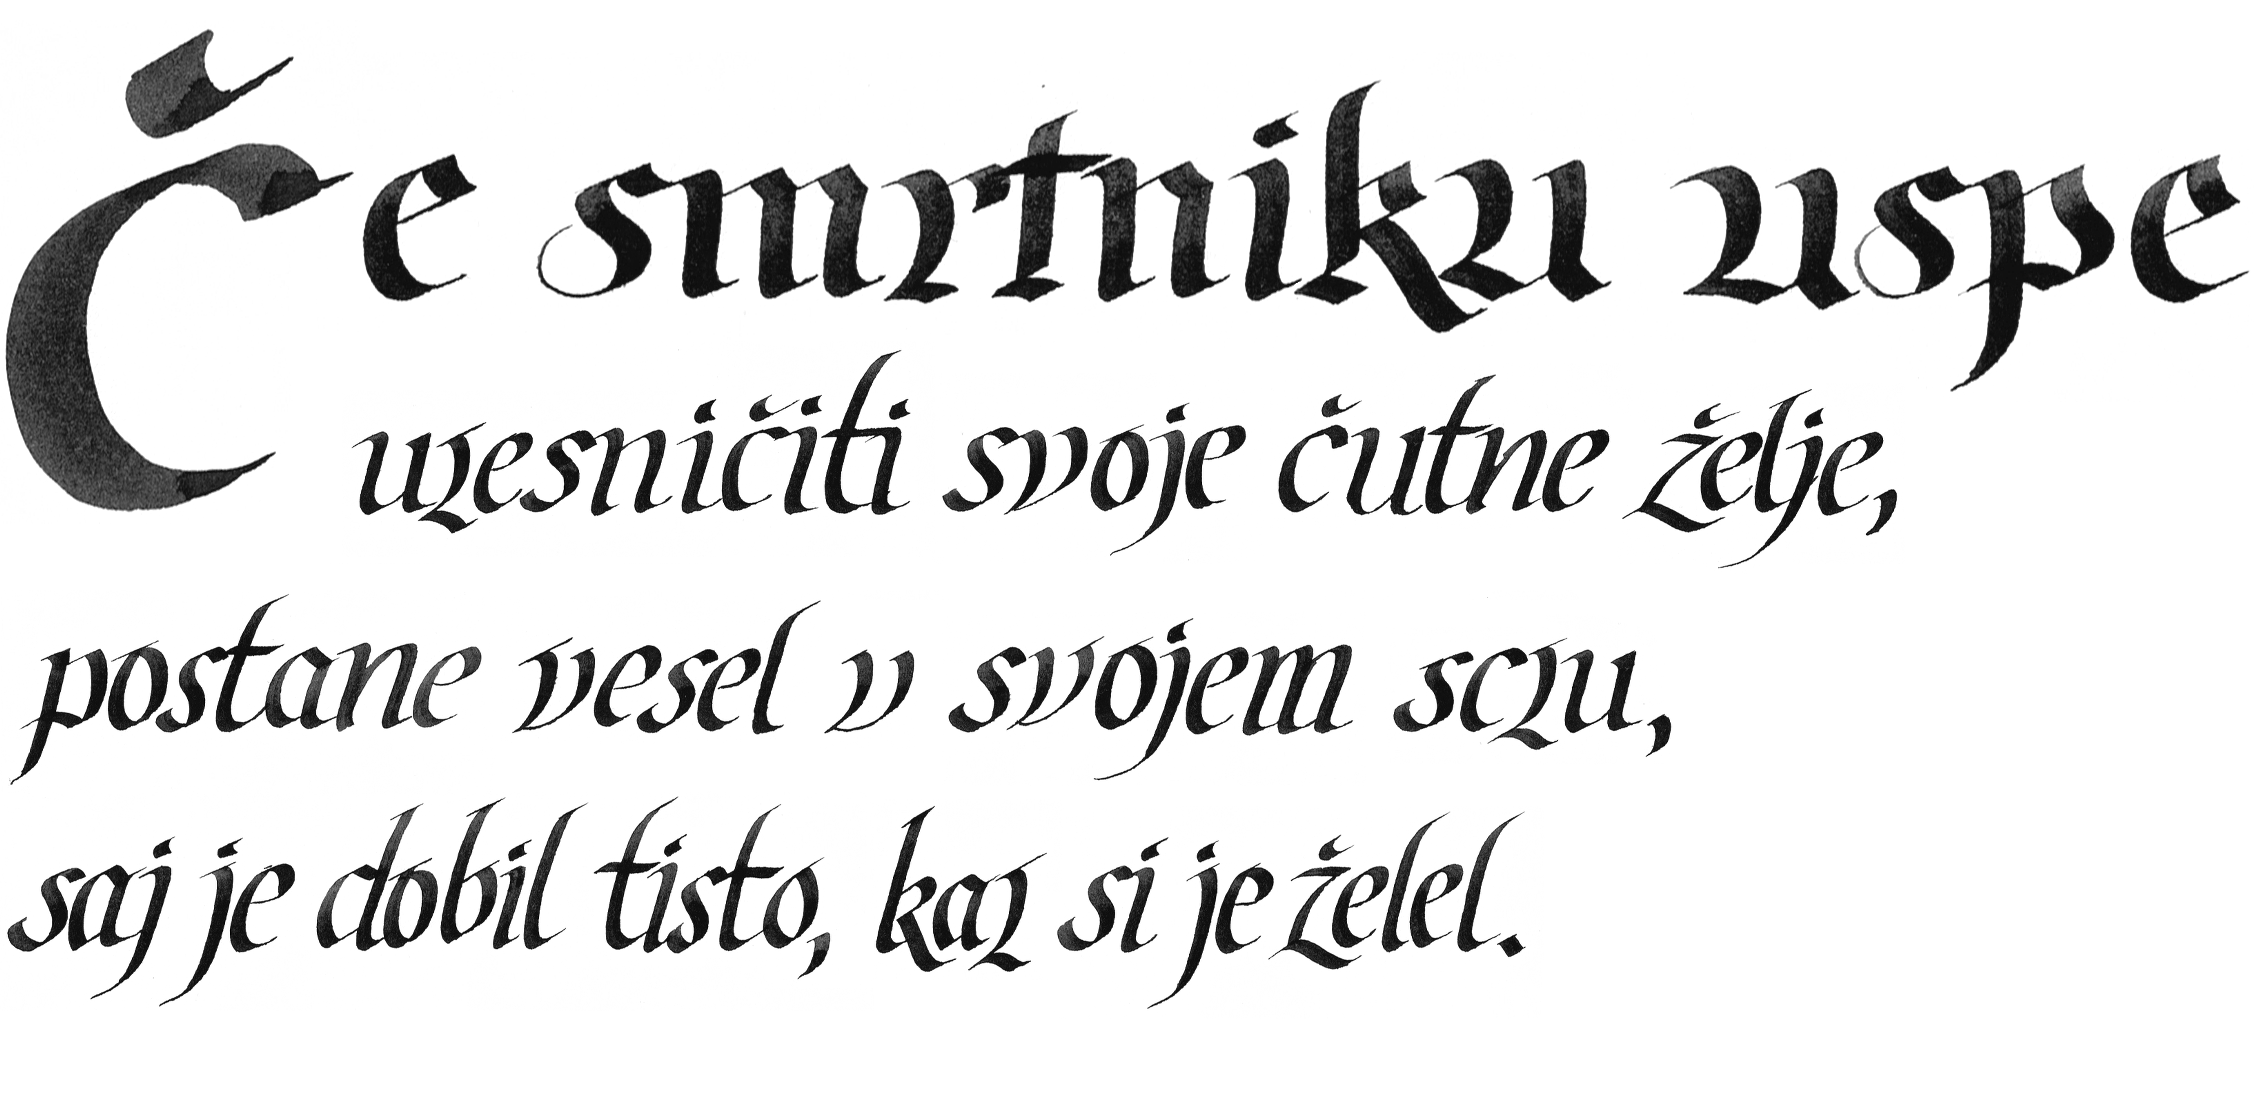
\includegraphics[scale=0.3]{ce-smrtniku-gray.png}

\verseref{1}
Spoznal sem hrepenenje, nezadovoljstvo in strast,\\
ne čutim več niti želja do spolnosti --\\
le kaj je to, polno urina in gnoja?\\
Tega se niti s svojo nogo ne bi hotel dotakniti.

\verseref{2}
\emph{Če si ne želite zaklada, kot je ta,\\
ženske, ki je zaželena med mnogimi gospodi,\\
kakšno prepričanje, moralo, običaje, način življenja,\\
in o kakšnem posmrtnem bivanju govorite?}

\verseref{3}
Tu ni ničesar, čemur bi lahko rekel: »To razglašam«, Māgandiya,\\
teorije, ki so bile prisvojene med ideologijami.\\
Vendar, ko sem brez oklepanja na njih opazoval poglede,\\
sem z razumevanjem spoznal notranji mir.

\verseref{4}
\emph{Katerakoli teorija se je oblikovala,\\
resnično, Modrijan, govorite o tem brez oklepanja.\\
Ta »notranji mir«, karkoli že to pomeni,\\
kako je ta spoznan med modrijani?}

\verseref{5}
Ne s tem, kar je bilo videno ali slišano, niti ne z znanjem, Māgandiya,\\
ne z moralo in običaji; reče se, da čistost je;\\
tudi ne z odsotnostjo tega, kar je videno ali slišano, niti ne z neznanjem,\\
brez morale in običajev -- tudi s tem ne.\\
Z opuščanjem tega, brez odvisnosti od česarkoli drugega,\\
miren človek, neodvisen, ne bo hrepenel po obstoju.

\verseref{6}
\emph{Če praviš, da se o čistosti ne govori s tem, kar je videno ali slišano,\\
niti ne z znanjem, ne z moralo in običaji;\\
tudi ne z odsotnostjo tega, kar je videno ali slišano, niti ne z neznanjem,\\
ne brez morale in običajev -- tudi s tem ne;\\
potem si predstavljam, da je to res zmedena ideologija.\\
Nekateri se zanašajo na čistost s pogledom.}

\verseref{7}
Zaradi takega spraševanja, ki je odvisno od pogledov, Māgandiya,\\
si postal zbegan s tem, ko si sebi prisvojil domneve.\\
Zato ne vidiš niti najmanjšega smisla v vsem tem\\
in vse to imaš za zmedo.

\verseref{8}
Kdor se ima za enakega, boljšega ali slabšega,\\
se bo boril glede na te oznake.\\
Tistemu, ki ne okleva med temi tremi razlikami,\\
se ne pojavljajo oznake »enak« ali »boljši«.

\verseref{9}
Čemu bi lahko ta sveti človek pravil: »To je resnica«,\\
ali se prepiral: »To je napačno«?\\
Za takega ni niti enakosti niti neenakosti --\\
le s kom bi se lahko prepiral?

\verseref{10}
Modrijan, ki je zapustil dom in je brez stalnega bivališča,\\
si ne gradi intime med ljudmi,\\
osvobodil se čutnih je užitkov, ničesar si ne postavlja v ospredje,\\
za nič se ne zavzema in ne razpravlja z ljudmi.

\verseref{11}
Od vseh stvari se je odrešil, med tem, ko še živi v tem svetu,\\
veliki človek se jih ne oklepa in se ne prepira.\\
Tako kot beli lokvanj, čigar pecelj raste iz vode\\
ni umazan z vodo in blatom,\\
tako tudi modrijan, govornik miru, človek brez pohlepa,\\
ni umazan s čutnostjo in svetom.

\verseref{12}
Tisti, ki je spoznal resnico v vidnem ali čutnem,\\
ni zato ošaben, saj se s tem ne enači.\\
Ne vodi ga, kar je bilo ustvarjeno ali naučeno,\\
in ne dela si zaključkov o tem, kar se je že uveljavilo.

\verseref{13}
Tu ni vezi za tistega, ki je nenavezan na zaznave,\\
tu ni zmedenosti za tistega, ki je osvobojen z razumevanjem.\\
Toda tisti, ki se močno oklepajo pogledov in zaznav,\\
pohajkujejo po svetu in povzročajo probleme.

\end{verse}

% === Pali ===

\clearpage
\begin{verse}

\verseref{5}

\end{verse}

% === Slovenian ===

\clearpage
\begin{verse}

\verseref{5}

\end{verse}

